\section{Failure modes visible only under simulation}
\label{sec:failures}

The model includes an automated director that plays the settlement without a
human: it lays networks, zones to demand, manages a budget and builds
structures. It is useful here as an instrument, because it exercises the model
in ways a scripted test does not --- and because its failures were failures of
the \emph{model's} reasoning, not of its code.

Four such failures were found by running complete settlement histories. All
four passed every placement test throughout, because placement was never what
was broken.

\subsection{Building what cannot be used}

The director initially treated a bore like any other terrain-gated structure:
site it wherever the terrain qualifies, the moment it is affordable. But
qualifying ground for a bore is, by construction, permanently shadowed crater
floor --- precisely the ground the settlement has no other reason to expand
toward. The director bought structures that its utility networks never reached,
and each sat at one level indefinitely: a completed purchase from the outside,
and worth nothing.

Over 900 simulated days on three seeds, the naive director built twelve
subsurface structures of which \textbf{one} ever grew (Figure~\ref{fig:dir}).

\subsection{Refusing is not the same as solving}

Requiring the utilities to reach a site before building eliminated the waste
entirely --- no stalled structures on any seed --- but at a cost: the director
now built only eight structures, because it would not go to the ice at all. The
lattice grows toward valuable ground, and shadowed floors are the least
valuable ground in the model, so it never arrived.

Only when the director was given an explicit reason to walk a corridor out to
the resource did both problems resolve: fourteen structures, all growing, none
stalled. The general lesson is that a resource which is valuable only
\emph{after} you have reached it will not be reached by an agent that expands
by local value alone. That is a statement about settlement dynamics, not about
this implementation.

\begin{figure}[htbp]
\centering
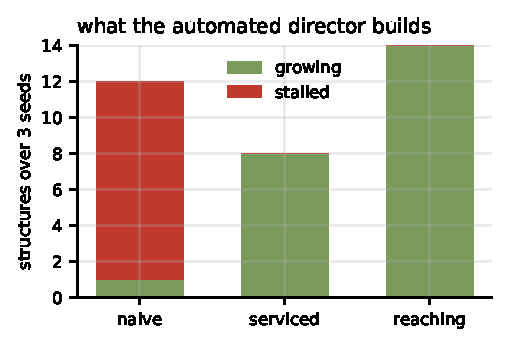
\includegraphics[width=0.5\textwidth]{figures/director-ab.pdf}
\caption{Subsurface structures built by three revisions of the automated
director over 900 simulated days on each of three seeds. The naive director
builds the most that never work.}
\label{fig:dir}
\end{figure}

\subsection{An adjacency predicate used for the wrong question}

The model asks "is this ground served by the power network?" using a predicate
that counts adjacency --- correct for deciding whether a tile may develop. The
corridor-building routine reused it to choose where to connect \emph{from},
which is a different question. A transit tube adjacent to a conduit reports
itself served and conducts nothing, so corridors anchored on one dead-ended a
single tile short, delivering transit and atmosphere to a structure with no
power.

The failure is instructive because every tile involved reported itself
correctly. Nothing was broken; a predicate was asked a question it does not
answer.

\subsection{A corridor that blocked its own successor}

Corridors laid a transit tube alongside the route for legibility. Excluding the
current route from that placement prevented a corridor from blocking itself,
but not from blocking a \emph{later} one: on one seed a site became ringed by
tubes left by its own abandoned attempts, could never be powered, and the
director re-laid the same two-tile corridor to it every 120 simulated days for
the remainder of the run.

This one is worth reporting for a methodological reason. On most of the seeds
swept during development the same defective revision built its full complement
of structures and looked entirely healthy; the fault appeared only on maps
where a corridor had to cross ground already occupied by an earlier attempt.
That is an argument for sweeping seeds rather than fixing one, and for
reporting a spread rather than a best case.

We flag explicitly that this observation, unlike the comparison in
Figure~\ref{fig:dir}, is \emph{not} among the recorded experiments. The
defective revision existed only in a working tree and was never committed, so
\texttt{e5-director-ab.mjs} --- which extracts its baselines by commit hash ---
cannot reproduce it. We report it because the failure mode is instructive, and
we mark it as unrecorded because it would otherwise carry an authority the
other results in this section have earned and it has not.

\subsection{A complexity failure hiding behind a logic failure}

Finally, the site-selection routine called a placement predicate that itself
scans the whole map, once per candidate tile --- quadratic in the map area.
This was harmless while the director placed a structure on the first tick it
could and then stopped looking. Once it was correctly refusing unreachable
sites, it never stopped looking, and the verification suite stopped completing
at all. The fix was to order the cheap network test before the expensive
placement test, reducing candidates from $16{,}384$ tiles to a few hundred.

A logic change turned a latent complexity bug into a fatal one without either
being visible in isolation. We report it because the interaction, not either
defect, is the interesting object.
